% Options for packages loaded elsewhere
\PassOptionsToPackage{unicode}{hyperref}
\PassOptionsToPackage{hyphens}{url}
%
\documentclass[
]{book}
\usepackage{amsmath,amssymb}
\usepackage{iftex}
\ifPDFTeX
  \usepackage[T1]{fontenc}
  \usepackage[utf8]{inputenc}
  \usepackage{textcomp} % provide euro and other symbols
\else % if luatex or xetex
  \usepackage{unicode-math} % this also loads fontspec
  \defaultfontfeatures{Scale=MatchLowercase}
  \defaultfontfeatures[\rmfamily]{Ligatures=TeX,Scale=1}
\fi
\usepackage{lmodern}
\ifPDFTeX\else
  % xetex/luatex font selection
\fi
% Use upquote if available, for straight quotes in verbatim environments
\IfFileExists{upquote.sty}{\usepackage{upquote}}{}
\IfFileExists{microtype.sty}{% use microtype if available
  \usepackage[]{microtype}
  \UseMicrotypeSet[protrusion]{basicmath} % disable protrusion for tt fonts
}{}
\makeatletter
\@ifundefined{KOMAClassName}{% if non-KOMA class
  \IfFileExists{parskip.sty}{%
    \usepackage{parskip}
  }{% else
    \setlength{\parindent}{0pt}
    \setlength{\parskip}{6pt plus 2pt minus 1pt}}
}{% if KOMA class
  \KOMAoptions{parskip=half}}
\makeatother
\usepackage{xcolor}
\usepackage{color}
\usepackage{fancyvrb}
\newcommand{\VerbBar}{|}
\newcommand{\VERB}{\Verb[commandchars=\\\{\}]}
\DefineVerbatimEnvironment{Highlighting}{Verbatim}{commandchars=\\\{\}}
% Add ',fontsize=\small' for more characters per line
\usepackage{framed}
\definecolor{shadecolor}{RGB}{248,248,248}
\newenvironment{Shaded}{\begin{snugshade}}{\end{snugshade}}
\newcommand{\AlertTok}[1]{\textcolor[rgb]{0.94,0.16,0.16}{#1}}
\newcommand{\AnnotationTok}[1]{\textcolor[rgb]{0.56,0.35,0.01}{\textbf{\textit{#1}}}}
\newcommand{\AttributeTok}[1]{\textcolor[rgb]{0.13,0.29,0.53}{#1}}
\newcommand{\BaseNTok}[1]{\textcolor[rgb]{0.00,0.00,0.81}{#1}}
\newcommand{\BuiltInTok}[1]{#1}
\newcommand{\CharTok}[1]{\textcolor[rgb]{0.31,0.60,0.02}{#1}}
\newcommand{\CommentTok}[1]{\textcolor[rgb]{0.56,0.35,0.01}{\textit{#1}}}
\newcommand{\CommentVarTok}[1]{\textcolor[rgb]{0.56,0.35,0.01}{\textbf{\textit{#1}}}}
\newcommand{\ConstantTok}[1]{\textcolor[rgb]{0.56,0.35,0.01}{#1}}
\newcommand{\ControlFlowTok}[1]{\textcolor[rgb]{0.13,0.29,0.53}{\textbf{#1}}}
\newcommand{\DataTypeTok}[1]{\textcolor[rgb]{0.13,0.29,0.53}{#1}}
\newcommand{\DecValTok}[1]{\textcolor[rgb]{0.00,0.00,0.81}{#1}}
\newcommand{\DocumentationTok}[1]{\textcolor[rgb]{0.56,0.35,0.01}{\textbf{\textit{#1}}}}
\newcommand{\ErrorTok}[1]{\textcolor[rgb]{0.64,0.00,0.00}{\textbf{#1}}}
\newcommand{\ExtensionTok}[1]{#1}
\newcommand{\FloatTok}[1]{\textcolor[rgb]{0.00,0.00,0.81}{#1}}
\newcommand{\FunctionTok}[1]{\textcolor[rgb]{0.13,0.29,0.53}{\textbf{#1}}}
\newcommand{\ImportTok}[1]{#1}
\newcommand{\InformationTok}[1]{\textcolor[rgb]{0.56,0.35,0.01}{\textbf{\textit{#1}}}}
\newcommand{\KeywordTok}[1]{\textcolor[rgb]{0.13,0.29,0.53}{\textbf{#1}}}
\newcommand{\NormalTok}[1]{#1}
\newcommand{\OperatorTok}[1]{\textcolor[rgb]{0.81,0.36,0.00}{\textbf{#1}}}
\newcommand{\OtherTok}[1]{\textcolor[rgb]{0.56,0.35,0.01}{#1}}
\newcommand{\PreprocessorTok}[1]{\textcolor[rgb]{0.56,0.35,0.01}{\textit{#1}}}
\newcommand{\RegionMarkerTok}[1]{#1}
\newcommand{\SpecialCharTok}[1]{\textcolor[rgb]{0.81,0.36,0.00}{\textbf{#1}}}
\newcommand{\SpecialStringTok}[1]{\textcolor[rgb]{0.31,0.60,0.02}{#1}}
\newcommand{\StringTok}[1]{\textcolor[rgb]{0.31,0.60,0.02}{#1}}
\newcommand{\VariableTok}[1]{\textcolor[rgb]{0.00,0.00,0.00}{#1}}
\newcommand{\VerbatimStringTok}[1]{\textcolor[rgb]{0.31,0.60,0.02}{#1}}
\newcommand{\WarningTok}[1]{\textcolor[rgb]{0.56,0.35,0.01}{\textbf{\textit{#1}}}}
\usepackage{longtable,booktabs,array}
\usepackage{calc} % for calculating minipage widths
% Correct order of tables after \paragraph or \subparagraph
\usepackage{etoolbox}
\makeatletter
\patchcmd\longtable{\par}{\if@noskipsec\mbox{}\fi\par}{}{}
\makeatother
% Allow footnotes in longtable head/foot
\IfFileExists{footnotehyper.sty}{\usepackage{footnotehyper}}{\usepackage{footnote}}
\makesavenoteenv{longtable}
\usepackage{graphicx}
\makeatletter
\def\maxwidth{\ifdim\Gin@nat@width>\linewidth\linewidth\else\Gin@nat@width\fi}
\def\maxheight{\ifdim\Gin@nat@height>\textheight\textheight\else\Gin@nat@height\fi}
\makeatother
% Scale images if necessary, so that they will not overflow the page
% margins by default, and it is still possible to overwrite the defaults
% using explicit options in \includegraphics[width, height, ...]{}
\setkeys{Gin}{width=\maxwidth,height=\maxheight,keepaspectratio}
% Set default figure placement to htbp
\makeatletter
\def\fps@figure{htbp}
\makeatother
\setlength{\emergencystretch}{3em} % prevent overfull lines
\providecommand{\tightlist}{%
  \setlength{\itemsep}{0pt}\setlength{\parskip}{0pt}}
\setcounter{secnumdepth}{5}
\usepackage{booktabs}
\usepackage{amsthm}
\makeatletter
\def\thm@space@setup{%
  \thm@preskip=8pt plus 2pt minus 4pt
  \thm@postskip=\thm@preskip
}
\makeatother
\ifLuaTeX
  \usepackage{selnolig}  % disable illegal ligatures
\fi
\usepackage[]{natbib}
\bibliographystyle{apalike}
\usepackage{bookmark}
\IfFileExists{xurl.sty}{\usepackage{xurl}}{} % add URL line breaks if available
\urlstyle{same}
\hypersetup{
  pdftitle={{[}PSY202B{]} Statistical Modeling in Psychological Sciences},
  pdfauthor={Ihnwhi Heo, M.Sc.},
  hidelinks,
  pdfcreator={LaTeX via pandoc}}

\title{{[}PSY202B{]} Statistical Modeling in Psychological Sciences}
\author{\href{https://ihnwhiheo.github.io/}{Ihnwhi Heo, M.Sc.}}
\date{Spring 2025}

\begin{document}
\maketitle

{
\setcounter{tocdepth}{1}
\tableofcontents
}
\chapter{Introduction}\label{introduction}

Hi everyone! I'm Ihnwhi.

It is my great pleasure to be your guest lecturer for PSY202B. The theme of my lecture is statistical modeling in psychological sciences.

An essential aspect of psychological research is statistical modeling based on substantive theories. It is thus important to use statistical software for accurate modeling to reach the research conclusion. I will briefly introduce Mplus and walk you around such analytic techniques as regression analysis, path analysis, confirmatory factor analysis, structural equation modeling (Part 1), and multilevel modeling (Part 2). This GitBook is your guide such that you can easily access code for Mplus.

Are you ready? Let's get it on!

\chapter{Introduction to Mplus}\label{introduction-to-mplus}

\section{What is it? Why called Mplus?}\label{what-is-it-why-called-mplus}

Mplus is a statistical modeling program that provides researchers with a flexible tool to analyze data

\begin{itemize}
\item
  Many models: regression, path analysis, factor analysis, SEM, MLM, longitudinal models, mixture model, mediation/moderation
\item
  Many data: cross-sectional, longitudinal, single-/multilevel, observed/latent, incomplete
\item
  Many variables: continuous, dichotomous, categorical, count
\item
  Many estimator: maximum likelihood, weighted least squares, Bayesian
\end{itemize}

\section{Syntax-based programming}\label{syntax-based-programming}

\begin{itemize}
\item
  Commands and subcommands (\url{https://www.statmodel.com/language.html})
\item
  Examples of commands? (\url{https://www.youtube.com/watch?v=XeRRtdmu23k})

  \begin{itemize}
  \tightlist
  \item
    We will be `mostly' using TITLE, DATA, VARIABLE, ANALYSIS, MODEL, OUTPUT commands
  \item
    But we will also be often using DEFINE, SAVEDATA, PLOT, MONTECARLO commands
  \end{itemize}
\end{itemize}

\section{Some tips when programming}\label{some-tips-when-programming}

\begin{enumerate}
\def\labelenumi{\arabic{enumi}.}
\item
  Comments can be added with exclamation marks (!)
\item
  Commands should end with colon (:), and subcommands should end with semicolon (;)
\item
  Syntax is not case sensitive
\item
  Data should consist of numeric values, with no variable names
\item
  Data and Mplus input file should be in the same directory (like an R working directory)
\end{enumerate}

\begin{itemize}
\tightlist
\item
  Otherwise, be sure to specify the correct directory
\end{itemize}

\section{Some tips about model command particularly}\label{some-tips-about-model-command-particularly}

\begin{enumerate}
\def\labelenumi{\arabic{enumi}.}
\item
  Start with a path diagram
\item
  Think of it as specifying model parameters
\item
  Care to the degrees of freedom (DF)
\end{enumerate}

\section{Example: Multiple linear regression using maximum likelihood estimation}\label{example-multiple-linear-regression-using-maximum-likelihood-estimation}

\subsection{Model syntax}\label{model-syntax}

\begin{Shaded}
\begin{Highlighting}[]
\SpecialCharTok{!}\NormalTok{ Title command}
\NormalTok{TITLE}\SpecialCharTok{:}\NormalTok{ Predicting album sales using ML multiple regression}

\SpecialCharTok{!}\NormalTok{ Data command}
\NormalTok{DATA}\SpecialCharTok{:}
    \SpecialCharTok{!}\NormalTok{ When data and input file are }\ControlFlowTok{in}\NormalTok{ the same working directory}
\NormalTok{    FILE IS Album Sales.csv; }\SpecialCharTok{!}\NormalTok{ Subcommands should end with ;}

    \SpecialCharTok{!}\NormalTok{ When data and input file are }\ControlFlowTok{in}\NormalTok{ the different working directory}
    \SpecialCharTok{!}\NormalTok{ FILE IS c}\SpecialCharTok{:}\NormalTok{\textbackslash{}desktop\textbackslash{}different folder\textbackslash{}Album Sales.csv;}

\SpecialCharTok{!}\NormalTok{ Variable command}
\NormalTok{VARIABLE}\SpecialCharTok{:}
    \SpecialCharTok{!}\NormalTok{ Column }\FunctionTok{names}\NormalTok{ (i.e., ALL variable names)}
\NormalTok{    NAMES ARE adverts sales airplay attract;}
    
    \SpecialCharTok{!}\NormalTok{ Variables that will be used }\ControlFlowTok{in}\NormalTok{ our analysis}
\NormalTok{    USEVARIABLES ARE adverts sales airplay;}
    
\SpecialCharTok{!}\NormalTok{ Analysis command}
\NormalTok{ANALYSIS}\SpecialCharTok{:}
\NormalTok{    ESTIMATOR IS ML; }\SpecialCharTok{!}\NormalTok{ This is the default}

\SpecialCharTok{!}\NormalTok{ Model command}
\NormalTok{MODEL}\SpecialCharTok{:}
    \SpecialCharTok{!}\NormalTok{ Let}\StringTok{\textquotesingle{}s predict sales using adverts and airplay}
\StringTok{    ! We regress sales on adverts and airplay}
\StringTok{    sales ON adverts airplay;}

\StringTok{    ! If you do not specify variances of and covariances between predictors}
\StringTok{    ! degrees of freedom (DF) are not correct}
\StringTok{    ! Variances of exogenous variable}
\StringTok{    adverts airplay;}
\StringTok{    ! Covariances between exogenous variable}
\StringTok{    adverts WITH airplay;}

\StringTok{! Output command}
\StringTok{OUTPUT:}
\StringTok{    TECH1 SAMPSTAT STDYX;}
\StringTok{    ! TECH1 to understand which parameters are being estimated}
\StringTok{    ! SAMPSTAT to check sample descriptive statistics}
\StringTok{    ! STDYX to standardize Y (i.e., DV) and X (i.e., IV)}
\end{Highlighting}
\end{Shaded}

\subsection{Part of the output file}\label{part-of-the-output-file}

\begin{Shaded}
\begin{Highlighting}[]
\NormalTok{MODEL RESULTS}

\NormalTok{                                                    Two}\SpecialCharTok{{-}}\NormalTok{Tailed}
\NormalTok{                    Estimate       S.E.  Est.}\SpecialCharTok{/}\NormalTok{S.E.    P}\SpecialCharTok{{-}}\NormalTok{Value}

\NormalTok{ SALES    ON}
\NormalTok{    ADVERTS            }\FloatTok{0.087}      \FloatTok{0.007}     \FloatTok{12.082}      \FloatTok{0.000}
\NormalTok{    AIRPLAY            }\FloatTok{3.589}      \FloatTok{0.285}     \FloatTok{12.608}      \FloatTok{0.000}

\NormalTok{ ADVERTS  WITH}
\NormalTok{    AIRPLAY          }\FloatTok{604.061}    \FloatTok{421.412}      \FloatTok{1.433}      \FloatTok{0.152}

\NormalTok{ Means}
\NormalTok{    ADVERTS          }\FloatTok{614.412}     \FloatTok{34.255}     \FloatTok{17.936}      \FloatTok{0.000}
\NormalTok{    AIRPLAY           }\FloatTok{27.500}      \FloatTok{0.865}     \FloatTok{31.777}      \FloatTok{0.000}
\end{Highlighting}
\end{Shaded}

\section{Additional materials}\label{additional-materials}

\begin{enumerate}
\def\labelenumi{\arabic{enumi}.}
\item
  Official website at \url{https://www.statmodel.com/}
\item
  User's guide and examples at \url{https://www.statmodel.com/ugexcerpts.shtml} \(\rightarrow\) Highly recommended!
\item
  Mplus YouTube channel at \url{https://www.youtube.com/c/MplusVideos}
\item
  QuantFish YouTube channel at \url{https://www.youtube.com/c/QuantFish}
\item
  Tutorials by Prof.~Rens van de Schoot and his students at \url{https://www.rensvandeschoot.com/tutorials/}
\end{enumerate}

\chapter{Path Analysis}\label{path-analysis}

\section{Research scenario}\label{research-scenario}

A team of researchers (Lucas, Alexis, Michelle, Fei, and Marisela) is interested in understanding the impact of anxiety and distress on hostile behavior. They are thus to conduct a path analysis to examine the interrelationships between the variables. According to the substantive theory, depression (\texttt{depress}) is predicted by anxiety (\texttt{anxiety}), and hostile behavior (\texttt{hostile}) is predicted by depression and distress. So here, depression is a mediating variable between anxiety and hostility. Two exogenous variables are anxiety and distress. Use the \texttt{mmpi.csv} dataset.

\section{Main questions}\label{main-questions}

\begin{enumerate}
\def\labelenumi{\arabic{enumi}.}
\item
  Draw a path diagram.
\item
  Write Mplus syntax.
\end{enumerate}

\begin{Shaded}
\begin{Highlighting}[]
\SpecialCharTok{!}\NormalTok{ Annotate what you are doing }\ControlFlowTok{in}\NormalTok{ this line}
\NormalTok{title}\SpecialCharTok{:}\NormalTok{ Path analysis}

\NormalTok{data}\SpecialCharTok{:}
\SpecialCharTok{!}\NormalTok{ Annotate what you are doing }\ControlFlowTok{in}\NormalTok{ this line}
\NormalTok{file is mmpi.csv;}

\NormalTok{variable}\SpecialCharTok{:}
\SpecialCharTok{!}\NormalTok{ Annotate what you are doing }\ControlFlowTok{in}\NormalTok{ this line}
\NormalTok{names are subid source age sex race slpneed slpget anxiety depress}
\NormalTok{hostile posafect senseek totaccpt totsavoid totici tottrust totmach}
\NormalTok{totpower totsms aggress impulse harm epixtra epineuro totrathus}
\NormalTok{totfaith totcyc totsd tothypo avoid distress;}

\SpecialCharTok{!}\NormalTok{ Annotate what you are doing }\ControlFlowTok{in}\NormalTok{ this line}
\NormalTok{usevariables are anxiety depress hostile distress;}

\NormalTok{analysis}\SpecialCharTok{:}
\SpecialCharTok{!}\NormalTok{ Annotate what you are doing }\ControlFlowTok{in}\NormalTok{ this line}
\NormalTok{estimator }\OtherTok{=}\NormalTok{ ML;}

\NormalTok{model}\SpecialCharTok{:}
\SpecialCharTok{!}\NormalTok{ Annotate what you are doing }\ControlFlowTok{in}\NormalTok{ this line}
\NormalTok{depress on anxiety;}

\SpecialCharTok{!}\NormalTok{ Annotate what you are doing }\ControlFlowTok{in}\NormalTok{ this line}
\NormalTok{hostile on depress;}

\SpecialCharTok{!}\NormalTok{ Annotate what you are doing }\ControlFlowTok{in}\NormalTok{ this line}
\NormalTok{hostile on distress;}

\SpecialCharTok{!}\NormalTok{ Annotate what you are doing }\ControlFlowTok{in}\NormalTok{ this line}
\NormalTok{anxiety;}

\SpecialCharTok{!}\NormalTok{ Annotate what you are doing }\ControlFlowTok{in}\NormalTok{ this line}
\NormalTok{distress;}

\SpecialCharTok{!}\NormalTok{ Annotate what you are doing }\ControlFlowTok{in}\NormalTok{ this line}
\NormalTok{anxiety with distress;}

\NormalTok{output}\SpecialCharTok{:}
\SpecialCharTok{!}\NormalTok{ Annotate what you are doing }\ControlFlowTok{in}\NormalTok{ this line}
\NormalTok{TECH1;}

\SpecialCharTok{!}\NormalTok{ Annotate what you are doing }\ControlFlowTok{in}\NormalTok{ this line}
\NormalTok{stdyx;}

\SpecialCharTok{!}\NormalTok{ Annotate what you are doing }\ControlFlowTok{in}\NormalTok{ this line}
\FunctionTok{modindices}\NormalTok{ (}\FloatTok{3.84}\NormalTok{);}
\end{Highlighting}
\end{Shaded}

\begin{enumerate}
\def\labelenumi{\arabic{enumi}.}
\setcounter{enumi}{2}
\tightlist
\item
  Run the analysis and interpret the results.
\end{enumerate}

\section{Bonus questions}\label{bonus-questions}

\begin{enumerate}
\def\labelenumi{\arabic{enumi}.}
\item
  Check the model fit. Are there any possibilities of improving model fit? Explore such possibilities using modification indices.
\item
  Calculate the degrees of freedom by hand. Compare your result with that of Mplus.
\end{enumerate}

\chapter{Confirmatory Factor Analysis}\label{confirmatory-factor-analysis}

\section{Research scenario}\label{research-scenario-1}

A team of developmental psychologists (Michelle, Lucas, and Alexis) is interested in constructing a psychometric theory on being manipulative to others. Our substantive theory suggests that sensation seeking (\texttt{senseek}), Machiavellianism (\texttt{totmach}), powerlessness (\texttt{totpower}), social monitoring (\texttt{totsms}), and faith (\texttt{totfaith}) measure the one underlying latent construct: being manipulative. We are thus to conduct a confirmatory factor analysis that measures manipulativeness by the five measures. Use the \texttt{mmpi.csv} dataset.

\section{Main questions}\label{main-questions-1}

\begin{enumerate}
\def\labelenumi{\arabic{enumi}.}
\item
  Draw a path diagram.
\item
  Write Mplus syntax.
\end{enumerate}

\begin{Shaded}
\begin{Highlighting}[]
\SpecialCharTok{!}\NormalTok{ Annotate what you are doing }\ControlFlowTok{in}\NormalTok{ this line}
\NormalTok{title}\SpecialCharTok{:}\NormalTok{ Confirmatory factor analysis}

\NormalTok{data}\SpecialCharTok{:}
\SpecialCharTok{!}\NormalTok{ Annotate what you are doing }\ControlFlowTok{in}\NormalTok{ this line}
\NormalTok{file is mmpi.csv;}

\NormalTok{variable}\SpecialCharTok{:}
\SpecialCharTok{!}\NormalTok{ Annotate what you are doing }\ControlFlowTok{in}\NormalTok{ this line}
\NormalTok{names are subid source age sex race slpneed slpget anxiety depress}
\NormalTok{hostile posafect senseek totaccpt totsavoid totici tottrust totmach}
\NormalTok{totpower totsms aggress impulse harm epixtra epineuro totrathus}
\NormalTok{totfaith totcyc totsd tothypo avoid distress;}

\SpecialCharTok{!}\NormalTok{ Annotate what you are doing }\ControlFlowTok{in}\NormalTok{ this line}
\NormalTok{usevariables are senseek totmach totpower totsms totfaith;}

\NormalTok{analysis}\SpecialCharTok{:}
\SpecialCharTok{!}\NormalTok{ Annotate what you are doing }\ControlFlowTok{in}\NormalTok{ this line}
\NormalTok{estimator }\OtherTok{=}\NormalTok{ ML;}

\NormalTok{model}\SpecialCharTok{:}
\SpecialCharTok{!}\NormalTok{ Annotate what you are doing }\ControlFlowTok{in}\NormalTok{ this line}
\NormalTok{manipulativeness BY senseek totmach totpower totsms totfaith;}

\SpecialCharTok{!}\NormalTok{ In case you want to free the first factor loading}
\SpecialCharTok{!}\NormalTok{ and instead scale the variance of the factor}
\SpecialCharTok{!}\NormalTok{ manipulativeness BY senseek}\SpecialCharTok{*}\NormalTok{ totmach totpower totsms totfaith;}
\SpecialCharTok{!}\NormalTok{ manipulativeness}\SpecialCharTok{@}\DecValTok{1}\NormalTok{;}

\NormalTok{output}\SpecialCharTok{:}
\SpecialCharTok{!}\NormalTok{ Annotate what you are doing }\ControlFlowTok{in}\NormalTok{ this line}
\NormalTok{TECH1;}

\SpecialCharTok{!}\NormalTok{ Annotate what you are doing }\ControlFlowTok{in}\NormalTok{ this line}
\NormalTok{stdyx;}
\end{Highlighting}
\end{Shaded}

\begin{enumerate}
\def\labelenumi{\arabic{enumi}.}
\setcounter{enumi}{2}
\tightlist
\item
  Run the analysis and interpret the results.
\end{enumerate}

\section{Bonus questions}\label{bonus-questions-1}

\begin{enumerate}
\def\labelenumi{\arabic{enumi}.}
\item
  By default, Mplus fixes the first factor loading to 1 for model identification. What if we want to free the first factor loading and instead scale the variance of the factor?
\item
  Calculate the degrees of freedom by hand. Compare your result with that of Mplus.
\end{enumerate}

\chapter{Structural Equation Modeling}\label{structural-equation-modeling}

\section{Research scenario}\label{research-scenario-2}

Based on the findings on the impact of anxiety and distress (Yepez et al., 2024; Gao et al., 2025; Reimers-Contreras \& Franco, 2023) and manipulative behavior (Parnell et al., 2024), Ihnwhi is interested in modeling the interrelationships between manipulativeness, anxiety, and distress. In particular, the research aim is to predict being manipulative using anxiety (\texttt{anxiety}) and distress (\texttt{distress}) via structural equation modeling. For the sake of convenience, you can only use the three following variables to measure manipulativeness: sensation seeking (\texttt{senseek}), Machiavellianism (\texttt{totmach}), and social monitoring (\texttt{totsms}). Use the \texttt{mmpi.csv} dataset.

\section{Main questions}\label{main-questions-2}

\begin{enumerate}
\def\labelenumi{\arabic{enumi}.}
\item
  Draw a path diagram.
\item
  Write Mplus syntax.
\end{enumerate}

\begin{Shaded}
\begin{Highlighting}[]
\SpecialCharTok{!}\NormalTok{ Annotate what you are doing }\ControlFlowTok{in}\NormalTok{ this line}
\NormalTok{title}\SpecialCharTok{:}\NormalTok{ Structural equation modeling}

\NormalTok{data}\SpecialCharTok{:}
\SpecialCharTok{!}\NormalTok{ Annotate what you are doing }\ControlFlowTok{in}\NormalTok{ this line}
\NormalTok{file is mmpi.csv;}

\NormalTok{variable}\SpecialCharTok{:}
\SpecialCharTok{!}\NormalTok{ Annotate what you are doing }\ControlFlowTok{in}\NormalTok{ this line}
\NormalTok{names are subid source age sex race slpneed slpget anxiety depress}
\NormalTok{hostile posafect senseek totaccpt totsavoid totici tottrust totmach}
\NormalTok{totpower totsms aggress impulse harm epixtra epineuro totrathus}
\NormalTok{totfaith totcyc totsd tothypo avoid distress;}

\SpecialCharTok{!}\NormalTok{ Annotate what you are doing }\ControlFlowTok{in}\NormalTok{ this line}
\NormalTok{usevariables are anxiety senseek totmach totsms distress;}

\NormalTok{analysis}\SpecialCharTok{:}
\SpecialCharTok{!}\NormalTok{ Annotate what you are doing }\ControlFlowTok{in}\NormalTok{ this line}
\NormalTok{estimator }\OtherTok{=}\NormalTok{ ML;}

\NormalTok{model}\SpecialCharTok{:}
\SpecialCharTok{!}\NormalTok{ Annotate what you are doing }\ControlFlowTok{in}\NormalTok{ this line}
\NormalTok{manipulativeness BY senseek totmach totsms;}

\SpecialCharTok{!}\NormalTok{ Annotate what you are doing }\ControlFlowTok{in}\NormalTok{ this line}
\NormalTok{manipulativeness on anxiety;}

\SpecialCharTok{!}\NormalTok{ Annotate what you are doing }\ControlFlowTok{in}\NormalTok{ this line}
\NormalTok{manipulativeness on distress;}

\SpecialCharTok{!}\NormalTok{ Annotate what you are doing }\ControlFlowTok{in}\NormalTok{ this line}
\NormalTok{anxiety;}

\SpecialCharTok{!}\NormalTok{ Annotate what you are doing }\ControlFlowTok{in}\NormalTok{ this line}
\NormalTok{distress;}

\SpecialCharTok{!}\NormalTok{ Annotate what you are doing }\ControlFlowTok{in}\NormalTok{ this line}
\NormalTok{anxiety with distress;}

\NormalTok{output}\SpecialCharTok{:}
\SpecialCharTok{!}\NormalTok{ Annotate what you are doing }\ControlFlowTok{in}\NormalTok{ this line}
\NormalTok{TECH1;}

\SpecialCharTok{!}\NormalTok{ Annotate what you are doing }\ControlFlowTok{in}\NormalTok{ this line}
\NormalTok{stdyx;}

\SpecialCharTok{!}\NormalTok{ Annotate what you are doing }\ControlFlowTok{in}\NormalTok{ this line}
\FunctionTok{modindices}\NormalTok{ (}\FloatTok{3.84}\NormalTok{);}
\end{Highlighting}
\end{Shaded}

\begin{enumerate}
\def\labelenumi{\arabic{enumi}.}
\setcounter{enumi}{2}
\tightlist
\item
  Run the analysis and interpret the results.
\end{enumerate}

\section{Bonus questions}\label{bonus-questions-2}

\begin{enumerate}
\def\labelenumi{\arabic{enumi}.}
\item
  Check the model fit. Are there any possibilities of improving model fit? Explore such possibilities using modification indices.
\item
  Can you interpret the TECH1 output given that the model formulation in Mplus is based on the LISREL ``all-y'' notation?
\end{enumerate}

\chapter{Multilevel Modeling}\label{multilevel-modeling}

\section{Multilevel data}\label{multilevel-data}

We have simulated data from 100 classes, with a different number of pupils in each class. The average class size is 20 pupils. On the pupil level, we have two variables. First is the dependent variable `popularity', measured on a self-rating scale that ranges from 0 (very unpopular) to 10 (very popular). Second is the independent variable `extraversion', measured on a self-rating scale ranging from 1 to 10. On the class level, we have one explanatory variable `teacher experience', measured in years ranging from 2 to 25.

\section{Building the multilevel regression model}\label{building-the-multilevel-regression-model}

We are to build three multilevel regression models in this practical. The three models to be built are as follows:

\begin{itemize}
\tightlist
\item
  Empty model (aka. intercept-only model)
\item
  Model with a level-1 predictor
\item
  Model with a level-2 predictor
\end{itemize}

For simplicity and illustrative purposes, we only consider random intercepts but not random slopes. On Wednesday, you will build the same three models in HLM software using a different dataset.

\section{Main questions}\label{main-questions-3}

\subsection{Empty model (aka. intercept-only model)}\label{empty-model-aka.-intercept-only-model}

\begin{enumerate}
\def\labelenumi{\arabic{enumi}.}
\tightlist
\item
  Write Mplus syntax.
\end{enumerate}

\begin{Shaded}
\begin{Highlighting}[]
\SpecialCharTok{!}\NormalTok{ Annotate what you are doing }\ControlFlowTok{in}\NormalTok{ this line}
\NormalTok{TITLE}\SpecialCharTok{:}\NormalTok{ Empty }\FunctionTok{model}\NormalTok{ (intercept}\SpecialCharTok{{-}}\NormalTok{only model)}

\NormalTok{DATA}\SpecialCharTok{:}
    \SpecialCharTok{!}\NormalTok{ Annotate what you are doing }\ControlFlowTok{in}\NormalTok{ this line}
\NormalTok{    file is popular2.dat;}

\NormalTok{VARIABLE}\SpecialCharTok{:}
    \SpecialCharTok{!}\NormalTok{ Annotate what you are doing }\ControlFlowTok{in}\NormalTok{ this line}
\NormalTok{    names are class pupil cons extrav sex texp popular popteach zextrav}
\NormalTok{    zsex ztexp zpopular zpoptch;}
    
    \SpecialCharTok{!}\NormalTok{ Annotate what you are doing }\ControlFlowTok{in}\NormalTok{ this line}
\NormalTok{    usevariables are popular;}
    
    \SpecialCharTok{!}\NormalTok{ Annotate what you are doing }\ControlFlowTok{in}\NormalTok{ this line}
\NormalTok{    cluster is class;}

\NormalTok{ANALYSIS}\SpecialCharTok{:}
    \SpecialCharTok{!}\NormalTok{ Annotate what you are doing }\ControlFlowTok{in}\NormalTok{ this line}
\NormalTok{    type is twolevel;}
    
    \SpecialCharTok{!}\NormalTok{ Annotate what you are doing }\ControlFlowTok{in}\NormalTok{ this line}
\NormalTok{    estimator is MLR;}

\NormalTok{MODEL}\SpecialCharTok{:}
    \SpecialCharTok{!}\NormalTok{ Annotate what you are doing }\ControlFlowTok{in}\NormalTok{ this line}
    \SpecialCharTok{\%within\%}

    \SpecialCharTok{!}\NormalTok{ Annotate what you are doing }\ControlFlowTok{in}\NormalTok{ this line}
    \SpecialCharTok{\%between\%}

\NormalTok{OUTPUT}\SpecialCharTok{:}
    \SpecialCharTok{!}\NormalTok{ Annotate what you are doing }\ControlFlowTok{in}\NormalTok{ this line}
\NormalTok{    sampstat cinterval;}
\end{Highlighting}
\end{Shaded}

\begin{enumerate}
\def\labelenumi{\arabic{enumi}.}
\setcounter{enumi}{1}
\item
  Run the analysis and interpret the results.
\item
  Can you match the parameter estimates to the notation in the formula below?
\end{enumerate}

\[
\begin{gathered}
\textbf{Level 1} \\ 
y_{ij}=\beta_{0j} + r_{ij} \\ \\
\textbf{Level 2} \\ 
\beta_{0j}=\gamma_{00} + u_{0j}
\end{gathered}
\]

\begin{enumerate}
\def\labelenumi{\arabic{enumi}.}
\setcounter{enumi}{3}
\tightlist
\item
  Can you compute the ICC?
\end{enumerate}

\subsection{Model with a level-1 predictor}\label{model-with-a-level-1-predictor}

\begin{enumerate}
\def\labelenumi{\arabic{enumi}.}
\tightlist
\item
  Write Mplus syntax.
\end{enumerate}

\begin{Shaded}
\begin{Highlighting}[]
\SpecialCharTok{!}\NormalTok{ Annotate what you are doing }\ControlFlowTok{in}\NormalTok{ this line}
\NormalTok{TITLE}\SpecialCharTok{:}\NormalTok{ Model with a level}\DecValTok{{-}1}\NormalTok{ predictor}

\NormalTok{DATA}\SpecialCharTok{:}
    \SpecialCharTok{!}\NormalTok{ Annotate what you are doing }\ControlFlowTok{in}\NormalTok{ this line}
\NormalTok{    file is popular2.dat;}

\NormalTok{VARIABLE}\SpecialCharTok{:}
    \SpecialCharTok{!}\NormalTok{ Annotate what you are doing }\ControlFlowTok{in}\NormalTok{ this line}
\NormalTok{    names are class pupil cons extrav sex texp popular popteach zextrav}
\NormalTok{    zsex ztexp zpopular zpoptch;}
    
    \SpecialCharTok{!}\NormalTok{ Annotate what you are doing }\ControlFlowTok{in}\NormalTok{ this line}
\NormalTok{    usevariables are extrav popular;}
    
    \SpecialCharTok{!}\NormalTok{ Annotate what you are doing }\ControlFlowTok{in}\NormalTok{ this line}
\NormalTok{    cluster is class;}
    
    \SpecialCharTok{!}\NormalTok{ Annotate what you are doing }\ControlFlowTok{in}\NormalTok{ this line}
\NormalTok{    within are extrav;}

\NormalTok{ANALYSIS}\SpecialCharTok{:}
    \SpecialCharTok{!}\NormalTok{ Annotate what you are doing }\ControlFlowTok{in}\NormalTok{ this line}
\NormalTok{    type is twolevel;}
    
    \SpecialCharTok{!}\NormalTok{ Annotate what you are doing }\ControlFlowTok{in}\NormalTok{ this line}
\NormalTok{    estimator is MLR;}

\NormalTok{MODEL}\SpecialCharTok{:}
    \SpecialCharTok{!}\NormalTok{ Annotate what you are doing }\ControlFlowTok{in}\NormalTok{ this line}
    \SpecialCharTok{\%within\%}
\NormalTok{    popular on extrav;}

    \SpecialCharTok{!}\NormalTok{ Annotate what you are doing }\ControlFlowTok{in}\NormalTok{ this line}
    \SpecialCharTok{\%between\%}
\NormalTok{    popular;}

\NormalTok{OUTPUT}\SpecialCharTok{:}
    \SpecialCharTok{!}\NormalTok{ Annotate what you are doing }\ControlFlowTok{in}\NormalTok{ this line}
\NormalTok{    sampstat cinterval;}

\NormalTok{SAVEDATA}\SpecialCharTok{:}
    \SpecialCharTok{!}\NormalTok{ Annotate what you are doing }\ControlFlowTok{in}\NormalTok{ this line}
\NormalTok{    file is fscores.dat;}
    
    \SpecialCharTok{!}\NormalTok{ Annotate what you are doing }\ControlFlowTok{in}\NormalTok{ this line}
\NormalTok{    save is fscores;}
\end{Highlighting}
\end{Shaded}

\begin{enumerate}
\def\labelenumi{\arabic{enumi}.}
\setcounter{enumi}{1}
\item
  Run the analysis and interpret the results.
\item
  Can you match the parameter estimates to the notation in the formula below?
\end{enumerate}

\[
\begin{gathered}
\textbf{Level 1} \\
y_{ij}=\beta_{0j} + \color{red}{\beta_{1j}X_{ij}} + r_{ij} \\ \\
\textbf{Level 2} \\
\beta_{0j}=\gamma_{00} + u_{0j} \\
\color{red}{\beta_{1j}=\gamma_{10}}
\end{gathered}
\]

\begin{enumerate}
\def\labelenumi{\arabic{enumi}.}
\setcounter{enumi}{3}
\tightlist
\item
  Can you compute the ICC?
\end{enumerate}

\subsection{Model with a level-2 predictor}\label{model-with-a-level-2-predictor}

\begin{enumerate}
\def\labelenumi{\arabic{enumi}.}
\tightlist
\item
  Write Mplus syntax.
\end{enumerate}

\begin{Shaded}
\begin{Highlighting}[]
\SpecialCharTok{!}\NormalTok{ Annotate what you are doing }\ControlFlowTok{in}\NormalTok{ this line}
\NormalTok{TITLE}\SpecialCharTok{:}\NormalTok{ Model with a level}\DecValTok{{-}2}\NormalTok{ predictor}

\NormalTok{DATA}\SpecialCharTok{:}
    \SpecialCharTok{!}\NormalTok{ Annotate what you are doing }\ControlFlowTok{in}\NormalTok{ this line}
\NormalTok{    file is popular2.dat;}

\NormalTok{VARIABLE}\SpecialCharTok{:}
    \SpecialCharTok{!}\NormalTok{ Annotate what you are doing }\ControlFlowTok{in}\NormalTok{ this line}
\NormalTok{    names are class pupil cons extrav sex texp popular popteach zextrav}
\NormalTok{    zsex ztexp zpopular zpoptch;}
    
    \SpecialCharTok{!}\NormalTok{ Annotate what you are doing }\ControlFlowTok{in}\NormalTok{ this line}
\NormalTok{    usevariables are texp popular;}
    
    \SpecialCharTok{!}\NormalTok{ Annotate what you are doing }\ControlFlowTok{in}\NormalTok{ this line}
\NormalTok{    cluster is class;}
    
    \SpecialCharTok{!}\NormalTok{ Annotate what you are doing }\ControlFlowTok{in}\NormalTok{ this line}
\NormalTok{    between are texp;}

\NormalTok{ANALYSIS}\SpecialCharTok{:}
    \SpecialCharTok{!}\NormalTok{ Annotate what you are doing }\ControlFlowTok{in}\NormalTok{ this line}
\NormalTok{    type is twolevel;}
    
    \SpecialCharTok{!}\NormalTok{ Annotate what you are doing }\ControlFlowTok{in}\NormalTok{ this line}
\NormalTok{    estimator is MLR;}

\NormalTok{MODEL}\SpecialCharTok{:}
    \SpecialCharTok{!}\NormalTok{ Annotate what you are doing }\ControlFlowTok{in}\NormalTok{ this line}
    \SpecialCharTok{\%within\%}
\NormalTok{    popular;}

    \SpecialCharTok{!}\NormalTok{ Annotate what you are doing }\ControlFlowTok{in}\NormalTok{ this line}
    \SpecialCharTok{\%between\%}
\NormalTok{    popular on texp;}

\NormalTok{OUTPUT}\SpecialCharTok{:}
    \SpecialCharTok{!}\NormalTok{ Annotate what you are doing }\ControlFlowTok{in}\NormalTok{ this line}
\NormalTok{    sampstat cinterval;}
\end{Highlighting}
\end{Shaded}

\begin{enumerate}
\def\labelenumi{\arabic{enumi}.}
\setcounter{enumi}{1}
\item
  Run the analysis and interpret the results.
\item
  Can you match the parameter estimates to the notation in the formula below?
\end{enumerate}

\[
\begin{gathered}
\textbf{Level 1} \\
y_{ij}=\beta_{0j} + r_{ij} \\ \\
\textbf{Level 2} \\
\beta_{0j}=\gamma_{00} + \color{red}{\gamma_{01}X_{j}} + u_{0j}
\end{gathered}
\]

\begin{enumerate}
\def\labelenumi{\arabic{enumi}.}
\setcounter{enumi}{3}
\tightlist
\item
  Can you compute the ICC?
\end{enumerate}

\section{Bonus questions}\label{bonus-questions-3}

\begin{enumerate}
\def\labelenumi{\arabic{enumi}.}
\tightlist
\item
  Can you visualize the results of multilevel modeling? Let's practice with the model with a level-1 predictor that we fitted.
\end{enumerate}

\begin{Shaded}
\begin{Highlighting}[]
\CommentTok{\# Clean the work space}
\FunctionTok{rm}\NormalTok{(}\AttributeTok{list=}\FunctionTok{ls}\NormalTok{()); }\FunctionTok{gc}\NormalTok{()}
\end{Highlighting}
\end{Shaded}

\begin{verbatim}
##          used (Mb) gc trigger (Mb) limit (Mb) max used (Mb)
## Ncells 501216 26.8    1097498 58.7         NA   669094 35.8
## Vcells 912551  7.0    8388608 64.0      16384  1839769 14.1
\end{verbatim}

\begin{Shaded}
\begin{Highlighting}[]
\CommentTok{\# Load required packages}
\FunctionTok{library}\NormalTok{(MplusAutomation)}
\end{Highlighting}
\end{Shaded}

\begin{verbatim}
## Warning: package 'MplusAutomation' was built under R version 4.2.3
\end{verbatim}

\begin{verbatim}
## Version:  1.1.1
## We work hard to write this free software. Please help us get credit by citing: 
## 
## Hallquist, M. N. & Wiley, J. F. (2018). MplusAutomation: An R Package for Facilitating Large-Scale Latent Variable Analyses in Mplus. Structural Equation Modeling, 25, 621-638. doi: 10.1080/10705511.2017.1402334.
## 
## -- see citation("MplusAutomation").
\end{verbatim}

\begin{Shaded}
\begin{Highlighting}[]
\FunctionTok{library}\NormalTok{(texreg)}
\end{Highlighting}
\end{Shaded}

\begin{verbatim}
## Version:  1.39.4
## Date:     2024-07-23
## Author:   Philip Leifeld (University of Manchester)
## 
## Consider submitting praise using the praise or praise_interactive functions.
## Please cite the JSS article in your publications -- see citation("texreg").
\end{verbatim}

\begin{Shaded}
\begin{Highlighting}[]
\FunctionTok{library}\NormalTok{(ggplot2)}
\end{Highlighting}
\end{Shaded}

\begin{verbatim}
## Warning: package 'ggplot2' was built under R version 4.2.3
\end{verbatim}

\begin{Shaded}
\begin{Highlighting}[]
\CommentTok{\# Extract fscores}
\NormalTok{out }\OtherTok{\textless{}{-}} \FunctionTok{readModels}\NormalTok{(}\StringTok{"2. Model with a l1 pred.out"}\NormalTok{, }\AttributeTok{recursive =} \ConstantTok{FALSE}\NormalTok{, }
                  \AttributeTok{what =} \StringTok{"savedata"}\NormalTok{)}
\NormalTok{fscores }\OtherTok{\textless{}{-}}\NormalTok{ out}\SpecialCharTok{$}\NormalTok{savedata}
\NormalTok{fscores\_classid }\OtherTok{\textless{}{-}} \FunctionTok{aggregate}\NormalTok{(fscores[,}\DecValTok{3}\SpecialCharTok{:}\DecValTok{4}\NormalTok{], }\FunctionTok{list}\NormalTok{(fscores}\SpecialCharTok{$}\NormalTok{CLASS), mean)}

\CommentTok{\# Check the range of the predictor}
\FunctionTok{range}\NormalTok{(fscores}\SpecialCharTok{$}\NormalTok{EXTRAV) }\CommentTok{\# 1 to 10}
\end{Highlighting}
\end{Shaded}

\begin{verbatim}
## [1]  1 10
\end{verbatim}

\begin{Shaded}
\begin{Highlighting}[]
\CommentTok{\# Find predicted values for each level of extraversion}
\NormalTok{pred\_popular\_classid }\OtherTok{\textless{}{-}} \FunctionTok{data.frame}\NormalTok{(fscores\_classid[}\FunctionTok{rep}\NormalTok{(}\FunctionTok{seq}\NormalTok{(}\FunctionTok{nrow}\NormalTok{(fscores\_classid)),}
                                                       \AttributeTok{each =} \DecValTok{10}\NormalTok{),],}
                                   \StringTok{"extraversion"} \OtherTok{=} \DecValTok{1}\SpecialCharTok{:}\DecValTok{10}\NormalTok{)}
\NormalTok{pred\_popular }\OtherTok{\textless{}{-}}\NormalTok{ pred\_popular\_classid}\SpecialCharTok{$}\NormalTok{B\_POPULAR }\SpecialCharTok{+} \FloatTok{0.486} \SpecialCharTok{*}\NormalTok{ pred\_popular\_classid}\SpecialCharTok{$}\NormalTok{extraversion}
\NormalTok{pred\_popular\_classid }\OtherTok{\textless{}{-}} \FunctionTok{data.frame}\NormalTok{(pred\_popular\_classid, pred\_popular)}

\CommentTok{\# Visualization}
\FunctionTok{ggplot}\NormalTok{(}\AttributeTok{data =}\NormalTok{ pred\_popular\_classid, }\FunctionTok{aes}\NormalTok{(}\AttributeTok{x =}\NormalTok{ extraversion, }\AttributeTok{y =}\NormalTok{ pred\_popular, }\AttributeTok{group =}\NormalTok{ Group}\FloatTok{.1}\NormalTok{)) }\SpecialCharTok{+}
  \FunctionTok{geom\_line}\NormalTok{(}\FunctionTok{aes}\NormalTok{(}\AttributeTok{color =}\NormalTok{ Group}\FloatTok{.1}\NormalTok{), }\AttributeTok{show.legend =} \ConstantTok{FALSE}\NormalTok{) }\SpecialCharTok{+}
  \FunctionTok{labs}\NormalTok{(}\AttributeTok{x =} \StringTok{"Extraversion"}\NormalTok{,}
       \AttributeTok{y =} \StringTok{"Popularity"}\NormalTok{) }\SpecialCharTok{+}
  \FunctionTok{scale\_y\_continuous}\NormalTok{(}\AttributeTok{lim =} \FunctionTok{c}\NormalTok{(}\DecValTok{0}\NormalTok{, }\DecValTok{10}\NormalTok{), }\AttributeTok{breaks =} \FunctionTok{seq}\NormalTok{(}\DecValTok{0}\NormalTok{, }\DecValTok{10}\NormalTok{, }\AttributeTok{by =} \DecValTok{1}\NormalTok{)) }\SpecialCharTok{+}
  \FunctionTok{scale\_x\_continuous}\NormalTok{(}\AttributeTok{lim =} \FunctionTok{c}\NormalTok{(}\DecValTok{1}\NormalTok{, }\DecValTok{10}\NormalTok{), }\AttributeTok{breaks =} \FunctionTok{seq}\NormalTok{(}\DecValTok{1}\NormalTok{, }\DecValTok{10}\NormalTok{, }\AttributeTok{by =} \DecValTok{1}\NormalTok{)) }\SpecialCharTok{+}
  \FunctionTok{theme\_bw}\NormalTok{()}
\end{Highlighting}
\end{Shaded}

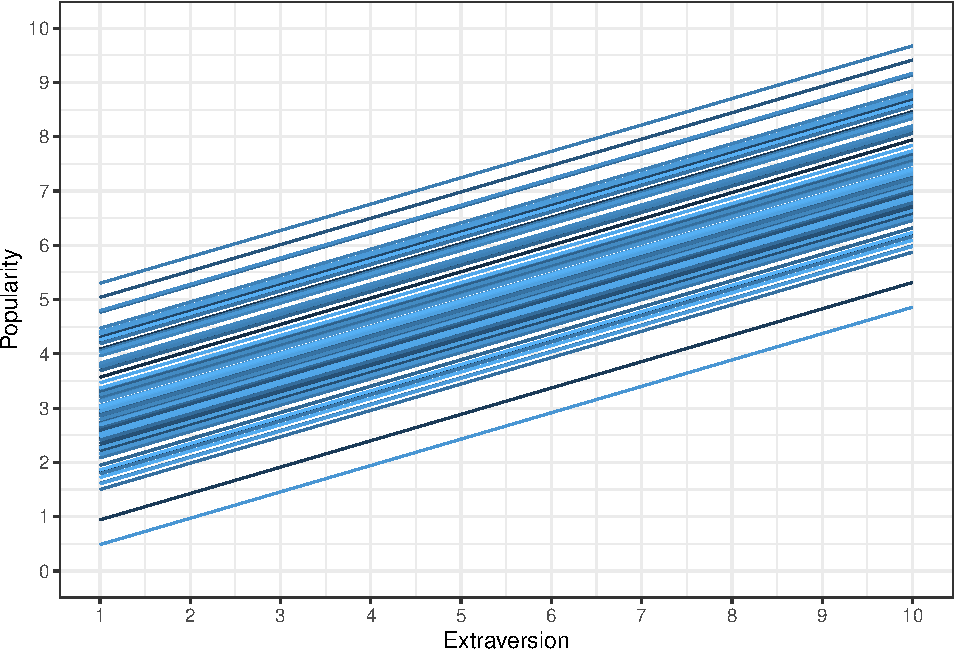
\includegraphics{PSY202B-Modeling-I.Heo_files/figure-latex/unnamed-chunk-9-1.pdf}

\begin{enumerate}
\def\labelenumi{\arabic{enumi}.}
\setcounter{enumi}{1}
\item
  How can you interpret the plot?
\item
  Can you imagine how the plot would look like when we consider random slopes?
\end{enumerate}

  \bibliography{book.bib,packages.bib}

\end{document}
